\documentclass[border=6pt]{standalone}
\usepackage{amsmath,amssymb}
\usepackage{xcolor}
\usepackage{tikz}
\usetikzlibrary{arrows.meta,decorations.pathreplacing,backgrounds}
\definecolor{cblue}{HTML}{1976D2}
\definecolor{cred}{HTML}{E53935}
\definecolor{cpurple}{HTML}{5E35B1}
\definecolor{cgrey}{HTML}{757575}
\tikzset{every picture/.append style={show background rectangle,
    background rectangle/.style={fill=white}, inner frame sep=4pt}}
% The ring buffer, drawn with h = 15 and W = 2: N = h + W + 3 = 20 samples, from k - h - 2 - W to the
% new sample k. The new sample completes the row of the start i = k - h, its distances to the samples
% at the lags of the window. The W + 2 samples before i hold the stretches of the undecided candidates.
\begin{document}
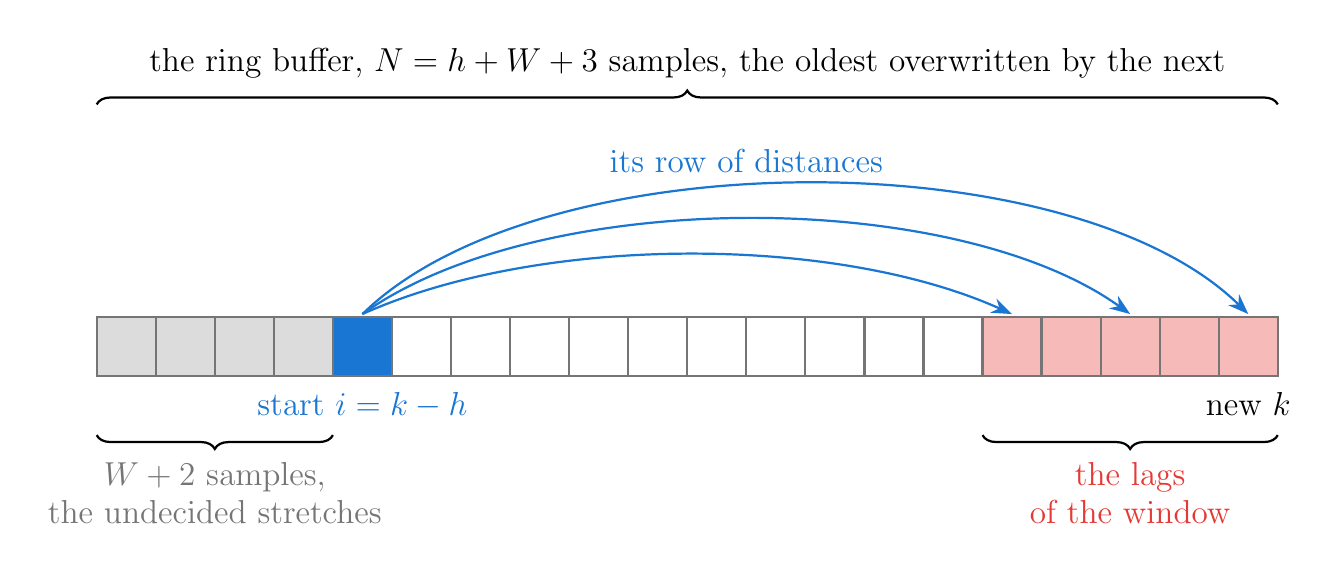
\begin{tikzpicture}[>={Stealth[length=2.6mm]}, every node/.style={font=\large}, x=0.75cm, y=0.75cm,
                    line width=0.8pt]
  % ---- the cells ----
  \foreach \k in {0,...,19} {
    \draw[cgrey, fill=white] (\k, 0) rectangle ++(1, 1);
  }
  \foreach \k in {0,...,3} { \draw[cgrey, fill=cgrey!25] (\k, 0) rectangle ++(1, 1); }
  \draw[cgrey, fill=cblue] (4, 0) rectangle ++(1, 1);
  \foreach \k in {15,...,19} { \draw[cgrey, fill=cred!35] (\k, 0) rectangle ++(1, 1); }

  % ---- the row of the start i, from it to three of the samples at its lags ----
  \draw[->, cblue] (4.5, 1.05) .. controls (7.5, 2.4) and (12.5, 2.4) .. (15.5, 1.05);
  \draw[->, cblue] (4.5, 1.05) .. controls (7.5, 3.2) and (14.5, 3.2) .. (17.5, 1.05);
  \draw[->, cblue] (4.5, 1.05) .. controls (7.5, 4.0) and (16.5, 4.0) .. (19.5, 1.05);
  \node[cblue] at (11.0, 3.65) {its row of distances};

  % ---- the labels under the cells ----
  \node[cblue, below] at (4.5, -0.1) {start $i = k - h$};
  \node[below] at (19.5, -0.1) {new $k$};
  \draw[decorate, decoration={brace, mirror, amplitude=5pt}] (0, -1.0) -- (4, -1.0)
      node[midway, below=6pt, cgrey, align=center] {$W + 2$ samples,\\ the undecided stretches};
  \draw[decorate, decoration={brace, mirror, amplitude=5pt}] (15, -1.0) -- (20, -1.0)
      node[midway, below=6pt, cred, align=center] {the lags\\ of the window};

  % ---- the whole buffer ----
  \draw[decorate, decoration={brace, amplitude=5pt}] (0, 4.6) -- (20, 4.6)
      node[midway, above=6pt] {the ring buffer, $N = h + W + 3$ samples, the oldest overwritten by the next};
\end{tikzpicture}
\end{document}
